\documentclass[12pt,a4paper]{article}
\usepackage[utf8]{inputenc}
\usepackage[czech]{babel}
\usepackage[T1]{fontenc}
\usepackage{amsmath}
\usepackage{amsfonts}
\usepackage{amssymb}
\usepackage{graphicx}
\usepackage{epstopdf}
\usepackage{indentfirst}
\setlength{\parindent}{4em} 
\author{Jakub Drápela}
\usepackage{fancyhdr}
\usepackage{siunitx}
\usepackage{pdflscape}
\usepackage[backend=bibtex,style=numeric]{biblatex}
\usepackage{filecontents}  % create "citations.bib" on-the-fly
\graphicspath{{./imgs/}}

%\fontfamily{phs}
%\selectfont

\begin{filecontents*}{podnik_zamer.bib}

@online{pict,
 author  = "The New York Times",
 title   = "The Amazon Echo",
 year    = "2015",
 urlseen = "03-17-16",
 url     = "http://static01.nyt.com/images/2015/06/25/business/GADGETWISE/GADGETWISE-master675.jpg",
}
\end{filecontents*}
\addbibresource{podnik_zamer.bib}

\begin{document}
\pagestyle{empty}

%%nastaveni pisma  
%\fontfamily{phv}
%\selectfont

	\begin{center}

\large

České vysoké učení technické v Praze

\medskip

Fakulta elektrotechnická 
\vfill
\vfill
{\LARGE\bfseries Household Intelligent Assistant}


\vspace{9mm}

\begin{figure}[h!]
\begin{center}
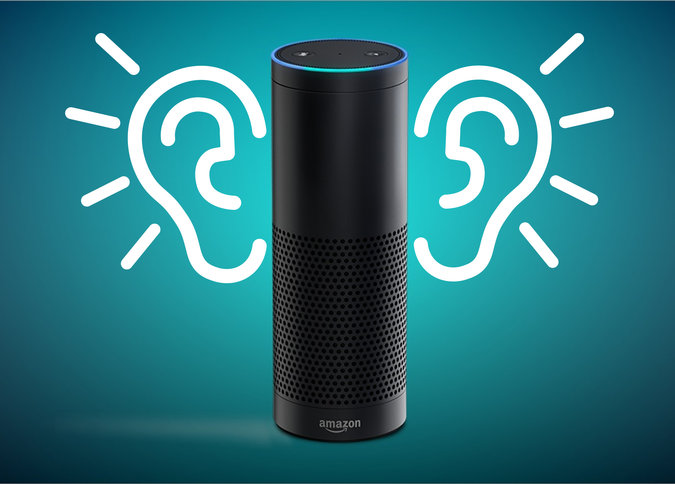
\includegraphics[width = 10cm]{ucho.jpg} 
\end{center}
\end{figure}

\vspace{9mm}

\begin{tabular}{rl}

Autoři: & Jiří Burant \\
\noalign{\vspace{1mm}}
		& Jakub Drápela \\
		\noalign{\vspace{1mm}}
		& Martin Klučka\\
		\noalign{\vspace{1mm}}
		& Petr Kovář \\
		\noalign{\vspace{1mm}}
		& Jakub Konrád\\
		\noalign{\vspace{1mm}}
		& Pavel Trutman\\
\noalign{\vspace{2mm}}
Studijní obor: & Kybernetika a robotika \\
\noalign{\vspace{2mm}}
Datum vypracování: & \today\\
\end{tabular}

\end{center}

\newpage
\pagestyle{plain}     % zapne obyčejné číslování
\setcounter{page}{1}
%% zahlaví a zápatí
\addtolength{\voffset}{-3cm}
\addtolength{\headheight}{2cm}

\pagestyle{fancy}
\lhead{
\includegraphics[scale=0.12]{cvut_text.jpg}  }
\rhead{\textbf{Household Intelligent Assistant}}
%\rhead{\textit{\bfseries Burant,Drápela,Klučka,Kovář,Konrád,Trutman}}
\lfoot{}
\cfoot{\thepage}
\rfoot{}
\renewcommand{\headrulewidth}{0.4pt}


\section*{Popis projektu, motivace}
Jako lidi si stále klademe různé otázky. Abychom mohli ve světě rozumně fungovat potřebujeme na tyto otázky znát odpovědi. Od té doby, co se začaly informace zaznamenávat lze odpovědi nalézt v záznamech. V nedávné historii lidé prahnoucí po informacích ve velkém kupovali knihy, noviny, jízdní řády, prostě média se žádaným obsahem. 

Doba pokročila a my jsme se posunuli do epochy, ve které jsou téměř všechny informace uložené v elektronické podobě. Je běžné k nim přistupovat pomocí moderních přístrojů. Téměř každý aktivní člověk vlastní alespoň jednu z věcí, jako je počítač, notebook, chytrý mobilní telefon, tablet, iPad a jiné. S využitím toho vybavení máme značně usnadněnou cestu k získání potřebné informace. Stačí mít u sebe správnou aplikaci, přístup na internet a například dopravní spojení nalezneme do minutky. V dnešní době nás limituje už jen to, že si požadovanou informaci musíme najít sami.

My se snažíme udělat krok vpřed. Ruční hledání informací obejít a nechat si informaci vyhledat automaticky nástrojem, který můžeme ovládat třeba jednoduše hlasem.

\section*{Detailní specifikace}
V našem projektu se zaměříme na vytvoření dialogového systému pro použití v běžné domácnosti či kanceláři. Tedy systému, který dovede sám odpovídat na kladené otázky z limitované oblasti počasí, dopravy, obecných informací atd. Systém bude neustále čekat na aktivační slovo a potom bude schopen zodpovědět určitou škálu otázek. K realizaci projektu použijeme již existující aplikace, které vhodně propojíme do funkčního celku.

V současné době existuje řada aplikací, které fungují na podobném principu. Uveďme například aplikaci \textbf{Cortana} od firmy Microsoft. Cortana, podobně jako další aplikace \textbf{Siri} od firmy Apple, je označována jako osobní asistent. Lze ji použít pro širokou škálu úkonů. Například hlasové ovládání přijímače nebo vyhledávání informací na internetu. Její nevýhodou je použití pouze pod operačním systémem Windows, případně iOS. 

Jako další lze uvést open-source aplikaci \textbf{Jasper} v jazyce Python. Tato aplikace umožňuje využití hlasu pro získání informací. Můžeme ji také použít v inteligentním bydlení a v dalších situacích. Jelikož je volně dostupná, lze k ní libovolně přidávat nové moduly a její použití ještě rozšířit. Stává se tak pro nás vhodnou inspirací. 

Za zmínku ještě stojí projekt \textbf{Amazon echo} od firmy Amazon. Tento osobní asistent z titulní strany umí přehrávat hudbu, odpovídat na otázky, vyhledávat zprávy, zjišťovat počasí, vytvářet seznamy a mnoho dalších věcí. 

My se budeme snažit o sestavení vlastního systému s podobnými vlastnostmi, jako mají již vzniklé projekty. 

\section*{Popis navrženého řešení}
Samotná finální aplikace se bude skládat z aplikačního jádra a modulů, které budou zodpovědné za jednotlivé funkcionality aplikace. Jádro aplikace bude pouze volat jednotlivé moduly a bude jim jen předávat získaná data z ostatních modulů. Bude tedy pouze řídit celý běh aplikace, ale nebude v něm probíhat žádné zpracování informací. Naopak jednotlivé moduly budou úzce zaměřené na zpracování nebo zjištění konkrétních dat. Mezi jádrem aplikace a jednotlivými moduly bude striktně definované rozhraní, což nám snadno umožní jednotlivé moduly nahradit za jiné, aniž by bylo třeba upravit jádro aplikace nebo ostatní moduly. Protože je aplikace vyvíjena jako otevřený software, umožňuje tato vysoká modularita každému uživateli jednoduše vytvořit si vlastní modul, případně si stávající modul upravit. Blokové schéma aplikace je zobrazeno na obrázku \ref{fig:diagram api}.

\begin{figure}[ht]
	\begin{center}
	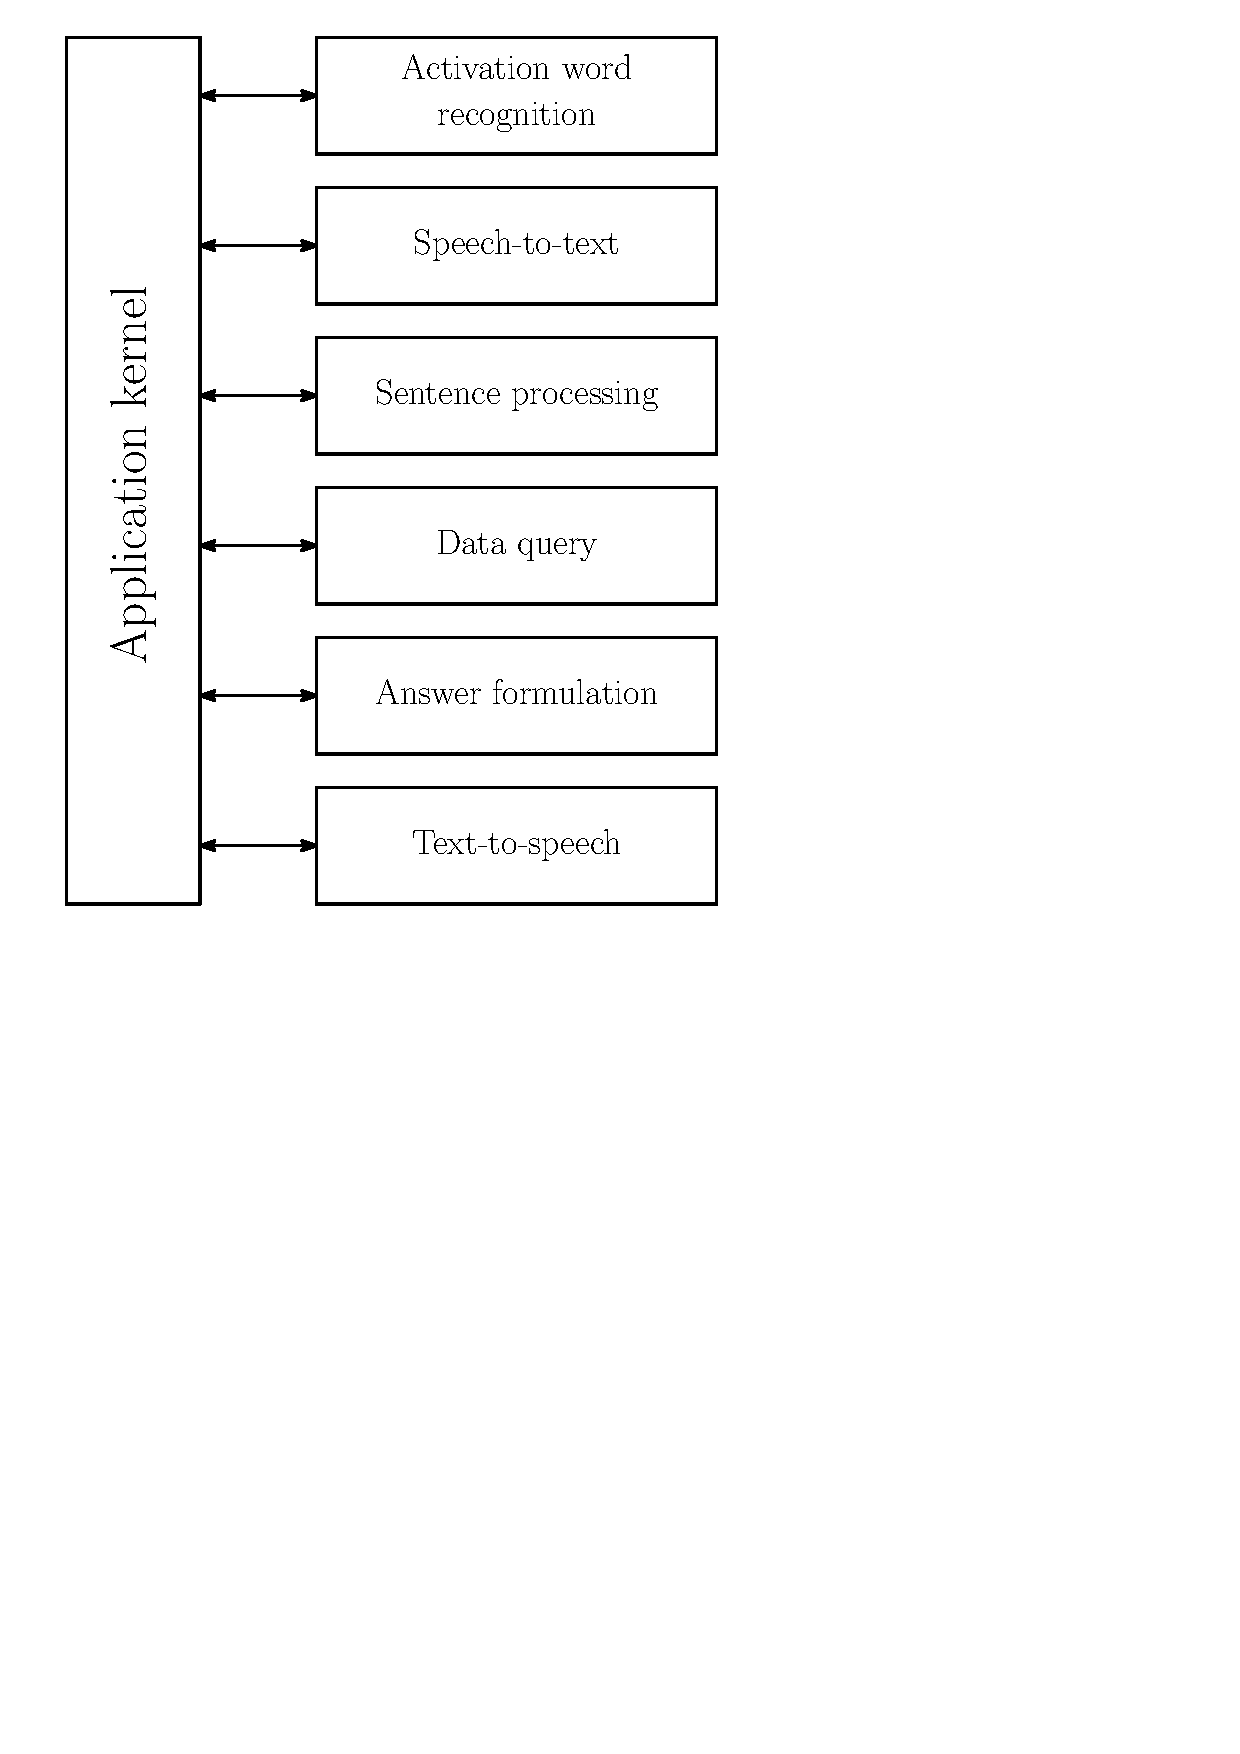
\includegraphics[height = 9cm]{blockDiagram.pdf}
	\caption{Blokový diagram navrženého řešení projektu Household Intelligent Assistant.}
	\label{fig:diagram api}
	\end{center}
\end{figure}

Při popisu návrhu řešení aplikace budeme postupovat tak, jak bude reakce na mluvené slovo postupně prostupovat mezi jednotlivými moduly, až nakonec vznikne finální řečená odpověď.

Za běžného provozu bude aplikace ve stand-by režimu, ve kterém bude čekat na zaznění aktivačního slova. Na rozpoznání aktivačního slova bude vyhrazen jeden samostatný modul. Aktivační slovo by mělo být snadno rozlišitelné od ostatních a zvukově velmi výrazné, aby nedocházelo k jeho záměně s hlukem na pozadí. Ukazuje se vhodné zvolit tříslabičné slovo s výraznými písmeny, jako jsou například písmena \uv{r} nebo \uv{x}.

Po zaznění aktivačního slova uživatelem se aktivuje blok pro rozpoznání mluveného slova, který převede položenou otázku na prostý text. Vhodnou robustní aplikací pro tento problém je třeba vybrat. Jako vhodné aplikace se ukazují třeba \textit{wit.ai} nebo \textit{PocketSphinx}. Tyto aplikace podrobněji prozkoumáme a vybereme tu, která se bude na daný problém lépe hodit.

Ze získaného textu z předchozího kroku je třeba vybrat klíčová slova, podle kterých určíme význam otázky. Klíčová slova umí rozeznávat, například již zmiňovaná, aplikace \textit{PocketSphinx}.

Získaná klíčová slova jsou vstupní hodnotou do modulu, jenž získá potřebné informace z internetu. Jednotlivé okruhy informací budou obstarávat jednotlivé subsystémy. Jeden subsystém bude například pouze na zpracování odpovědi na počasí, třeba přes aplikaci \textit{forecast.io}.

Informace získané z internetu je třeba přeformulovat do srozumitelné odpovědi podle předem zadaných vzorů. To bude úkolem dalšího samostatného modulu.

V poslední řadě využijeme aplikaci k převedení formulované odpovědi do strojově mluvené řeči. Prvotní aplikací pro tento převod může být jednoduchý \textit{"The Festival Speech Synthesis System"}. Později můžeme použít jinou aplikaci, která má převod textu na řeč více propracovanější.

% plus dopsat nějaké kecy kolem 

\section*{Plánování projektu}
Při plánování projektu je nutné vytvořit časový plán projektu neboli harmonogram, který obsahuje naplánovanou posloupnost jednotlivých činností s datem jejich plnění a klíčové milníky. Harmonogram projektu je graficky znázorněn formou Ganttova diagramu na obr. \ref{fig:diagram gantt}. Ganttův diagram zobrazuje ve sloupcích časové období a v řádcích jednotlivé plány. 

\begin{landscape}
\begin{figure}[ht]
	\begin{center}
	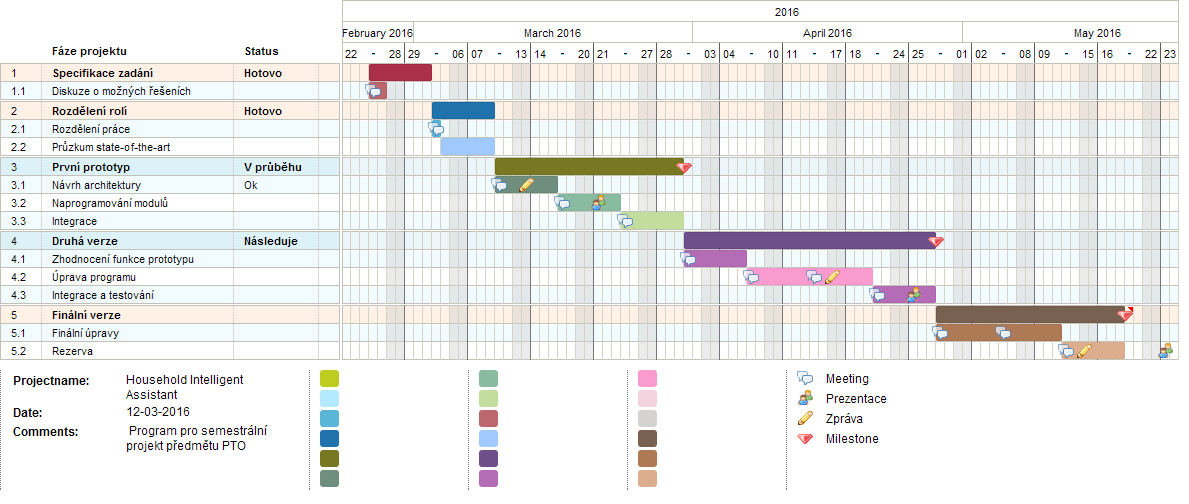
\includegraphics[height = 0.6\textheight ]{PTO-Gantt.png}
	\caption{Harmonogram projektu graficky znázorněn formou Ganttova diagramu s klíčovými milníky. Obsahuje pět stěžejních fází projektu. 
První dvě fáze projektu, diskutování nad řešením projektu a rozdělení rolí v týmu, jsme si již vyjasnili. Následuje realizace prvotního prototypu s omezenými schopnostmi. Prototyp následně postoupí fázi rozšiřování o nové možnosti a v poslední řadě přichází na řadu testování a finální úprava.}
	\label{fig:diagram gantt}
	\end{center}
\end{figure}
\end{landscape}

Časový plán projektu zahrnuje, kromě časového rozložení jednotlivých úkolů a milníků, také pravidelné týdenní schůze, termíny odevzdání průběžných zpráv a prezentace stavu projektu.


\section*{Analýza rizik a krizové plány}
V průběhu řešení projektu mohou nastat situace, jenž budou nepříjemnou překážkou v realizaci projektu. V nejhorším případě zapříčiní jeho zkázu. S riziky je třeba počítat a připravit si pro ně odpovídající krizové plány. Lze se tak vyvarovat zbytečných zmatků, vzniklé problémy efektivně řešit a minimalizovat tak jejich následky. \\

\noindent \textbf{Rizika projektu}, která mohou nastat a \textbf{plány} na jejich eliminaci: 

\begin{itemize}
	\item{\textbf{Nedostatečná funkčnost některého z modulů}} - jednotlivé moduly, které využívají již existující aplikace nebudou mít dostatečnou funkčnost.
	
	Podobných aplikací je na internetu spousta. Je zapotřebí vhodnými experimenty nalézt takovou, která bude dostatečně odpovídat kladeným požadavkům. Nebude-li taková aplikace existovat, budeme muset si chybějící funkcionalitu naprogramovat sami.
	
	\item{\textbf{Nemoc}} - v dlouhodobém řešení projektu zastihne některého člena týmu vážná nemoc. 
	
	V tomto případě zastoupí nemocného člena jiný člen a práce se přeorganizuje tak, aby nevznikaly zbytečné prodlevy. Obdobně budeme jednat, pokud někdo z týmu nebude stíhat plnit zadanou práci, ať už se jedná o jakýkoliv důvod. 
	
	\item{\textbf{Finance}} - nebude k dispozici dostatek financí.
	
	Budeme využívat volně dostupných programů. Nebude tak potřeba žádná investice.
	
	\item{\textbf{Ztráta dat}} - vlivem selhání lidského faktoru nebo elektroniky dojde ke ztrátě kódu a dat.
	
	Data je třeba zálohovat. Proto si vytvoříme repozitář na serveru GitHub, kam budou mít všichni členové přístup a budou zde průběžně ukládat svoji práci. Na serveru vždy bude uložena aktuální verze projektu s celou jeho historií, navíc každý uživatel bude mít u sebe jeho lokální kopii. Riziko se tak sníží téměř k nule. 
	
	\item{\textbf{Špatná komunikace}} - nedostatečná komunikace mezi členy týmu, což může vést ke zbytečnému nedorozumění. 
	
	Pravidelné týdenní schůzky pomáhají ve vyjasnění věcí, které nebyly zřejmé. Všichni členové týmu se navíc pravidelně potkávají ve škole díky studiu stejných předmětů, kde mohou hodně věcí probrat. Členové týmu jsou tak mezi sebou v kontaktu takřka denně. Další vhodnou komunikací je společenský webový systém \textit{Facebook}, který téměř všichni členové týmu využívají.
	
	\item{\textbf{Nerealistické termíny}} - určíme si cíl projektu, který není možné za daných okolností stihnou včas.
	
	Na počátku si naplánujeme postup práce a zkonzultujeme jej se všemi členy týmu a s vedoucím skupiny. Zhotovíme si Ganttův diagram (viz obr. \ref{fig:diagram gantt}), kterým se budeme řídit.
	
	\item{\textbf{Nedostatečné či neúplné testování}} - vznikne finální verze, která nebude dostatečně odzkoušená a bude obsahovat skryté vady.
	
	Včas dokončíme podstatné části projektu a vyhradíme si čas na jejich testování, které budeme provádět systematicky. Jednotlivé komponenty systému budeme testovat zvlášť po každém přidání nebo úpravě funkcionality. Závěrem budeme testovat celý systém jako celek. K testování systému pozveme i jiné osoby než jen členy týmu. 
	
	 
	
\end{itemize}



\section*{Předběžné výsledky}


\nocite{*}
\printbibliography 

\end{document}
